\documentclass[11pt]{article}
\usepackage[letterpaper,margin=1in]{geometry}
\usepackage[T1]{fontenc}
\usepackage[utf8]{inputenc}
\usepackage{amsmath}
\usepackage{newtxtext,newtxmath}
\usepackage[varqu,varl,scaled=0.95]{zi4}
\usepackage{microtype}
\usepackage{graphicx}
\graphicspath{{figures/}}  % figures/ or flat next to main.tex (e.g. an Overleaf upload)
\usepackage{booktabs,tabularx,array,xcolor,longtable,xltabular}
\setlength{\LTpre}{5pt}\setlength{\LTpost}{5pt}
\usepackage{flafter}  % floats never land above their definition (longtable-safe)
\setcounter{topnumber}{3}\setcounter{bottomnumber}{2}\setcounter{totalnumber}{4}
\renewcommand{\topfraction}{0.85}\renewcommand{\bottomfraction}{0.6}
\renewcommand{\textfraction}{0.12}\renewcommand{\floatpagefraction}{0.75}
\usepackage{enumitem}
\setlist{nosep,leftmargin=1.4em,topsep=3pt}
\usepackage{algorithm}
\usepackage{algpseudocode}
\usepackage[numbers,sort&compress]{natbib}
\usepackage{caption}
\captionsetup{font=small,labelfont=bf}
\usepackage{newunicodechar}
\definecolor{linkblue}{HTML}{1F4FD8}
\usepackage[colorlinks,linkcolor=linkblue,citecolor=linkblue,urlcolor=linkblue,unicode]{hyperref}
\usepackage{url}
\renewcommand{\arraystretch}{1.12}
\renewcommand{\bibfont}{\small\raggedright}
\setlength{\bibsep}{3pt}
\newcolumntype{L}{>{\raggedright\arraybackslash}X}
\newcommand{\nl}{\texttt{\textbackslash n}}
\newcommand{\code}[1]{\texttt{#1}}
\newunicodechar{−}{\ensuremath{-}}
\newunicodechar{≈}{\ensuremath{\approx}}
\newunicodechar{Δ}{\ensuremath{\Delta}}
\newunicodechar{×}{\ensuremath{\times}}
\newunicodechar{≤}{\ensuremath{\le}}
\newunicodechar{≥}{\ensuremath{\ge}}
\newunicodechar{→}{\ensuremath{\to}}
\newunicodechar{τ}{\ensuremath{\tau}}
\newunicodechar{β}{\ensuremath{\beta}}
\newunicodechar{λ}{\ensuremath{\lambda}}
\newunicodechar{ε}{\ensuremath{\varepsilon}}
\newunicodechar{·}{\ensuremath{\cdot}}
\newunicodechar{∀}{\ensuremath{\forall}}
\newunicodechar{⇒}{\ensuremath{\Rightarrow}}
\newunicodechar{∞}{\ensuremath{\infty}}
\newunicodechar{⟨}{\ensuremath{\langle}}
\newunicodechar{⟩}{\ensuremath{\rangle}}
\newunicodechar{∈}{\ensuremath{\in}}
\newunicodechar{∪}{\ensuremath{\cup}}
\newunicodechar{⊇}{\ensuremath{\supseteq}}
\newunicodechar{†}{\textsuperscript{\textdagger}}

\title{Beam Search Is Optional: Certified, Late-Entry Decoding for LLM Generative Recommenders}
\author{Authors to be added}
\date{\small Working draft, 2026-11-13. Every number cites a run under \code{runs/\allowbreak{}} (GPU named in each table).}
\begin{document}
\maketitle
\begin{abstract}
LLM-based generative recommenders emit an item as a short semantic-ID (SID) token sequence under a catalog trie and serve it with constrained beam search. On an open, widely reproduced instance — MiniOneRec (Qwen2-1.5B, three-level SIDs) on its two released datasets — we replace beam search with \textbf{certified exact decoding}: one tree-attention forward over the prompt and every first-level trie node bounds every catalog item (all scored terms are log-probabilities ≤ 0), a second forward over the best-bounded prefixes yields exact scores, and an on-device test certifies that the returned top-K is the global optimum of the model's objective (0 violations against brute force; 100\% of requests certified). The certificate itself is classical (exact n-best search, Fagin's threshold algorithm) and was recently stated for generative recommendation as a post-hoc beam completion; we make it the decoder and show what makes it cheap. Under \textbf{trie normalization} the bounds are two-sided — the best child of a prefix with n children scores at least −log n — so the set of prefixes to expand is known, and certification guaranteed, right after the first forward; that set averages ≤ 1.1·K prefixes at every K up to 500 and is within 1.2–2.1× of the provable minimum for any bound-based decoder. On synthetic catalogs of up to 1M SIDs on the same model, the minimal expansion stays flat (≈8 prefixes for a certified top-10) and so does latency at a fixed budget. We further find that \textbf{deeper SID codes do not need the lower layers}: prefix rows \emph{enter} the second forward at layer 26 of 28 (first-level rows at layer 18) from small bridges distilled from the parent node's state on the frozen model (validation prompts only, no labels), losslessly against the full-depth model (ΔHR@10 +0.12 [−0.27, +0.51], ΔNDCG@10 0.00 [−0.20, +0.20]). With a hand-written engine (one CUDA graph per request), a certified top-10 takes \textbf{2.75 ms on an H100} (MiniOneRec's beam-50 in the same engine and allocation: 8.43 ms; Hugging Face \code{generate}: 869 ms on an A6000), and a certified top-500 2.92 ms (beam-500: 18.1 ms). On the same H100 and workload, FlashRec, a public engine built for SID decoding (CUDA-graph wide beam, fused trie kernel), takes 11.5 ms per request and serves ≤ 0.5k users/s; certified decoding serves 2.7k (FP16) to 3.1k (FP8) users/s, while the two engines run beam search at the same throughput. Exact search also makes \textbf{objective fusion exact}: adding a per-user collaborative term (β·log q from a 1-minute SASRec, itself computed inside the same CUDA graph: 2.89 ms end to end) inside the certified search keeps two forwards and 100\% certification and raises Office HR@10 from 0.1714 to \textbf{0.1825} (+1.11 [+0.62, +1.60]; +2.36 points over MiniOneRec's FP32 beam decode of the same checkpoint, with no LLM training) and HR@500 by \textbf{4.0 points}, where beam-then-rerank cannot change the candidate set; Industrial gains +0.51 [+0.07, +0.95]. With random item values, beam-then-rerank recovers only 50\% of the exact top-10. One more epoch of supervised fine-tuning adds +0.8 HR@10 (+2.0 HR@50) to the released checkpoint — but matching the training loss to the decoder's normalization adds nothing beyond a full-vocabulary control. Dynamic per-token FP8 is quality-neutral and adds 16–21\% throughput; custom weight-streaming GEMMs, a one-forward variant with in-flight prefix selection, and weight-only INT8 do not help at these shapes.
\end{abstract}

\section{Introduction}\label{sec:1}

Generative retrieval with semantic IDs is deployed at scale (OneRec~\cite{ax2506.13695}, GR4AD~\cite{ax2602.22732}, GRACE~\cite{ax2608.00938}, PinRec~\cite{ax2504.10507}, Spotify~\cite{spotify2026}, NVIDIA SID-GR~\cite{nvidiasidgr}) and serving cost gates its use. Public engines report throughput against SGLang/vLLM/TensorRT-LLM with \emph{approximate} parity (FlashRec~\cite{flashrec}: 86–92\% beam-set overlap; NVIDIA: top-K overlap 0.96) and make silent, different scoring choices (full-vocabulary log-softmax then mask; per-codebook softmax; mask-before-softmax; \code{ignore\_\allowbreak{}eos}). We ask, on one fully reproducible model family with two datasets:

\begin{figure}[htp]
\centering
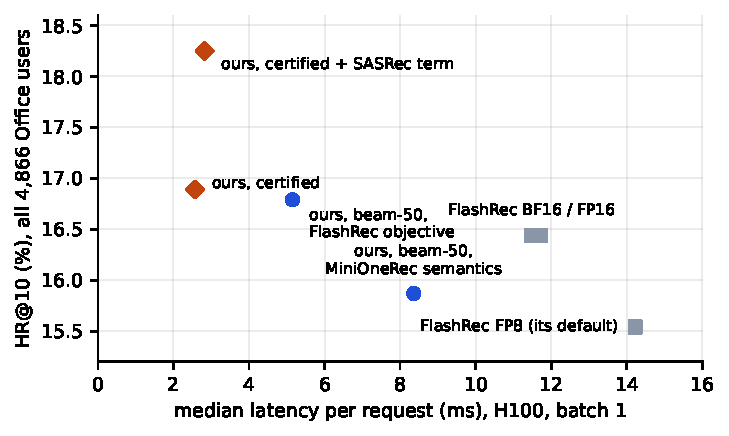
\includegraphics[width=0.62\linewidth]{h100_latency_quality.pdf}
\caption{Latency and quality on one H100 (Office, batch 1, median over $2\times500$ requests, one allocation, \code{runs/frLat}). FlashRec is the public SID-GR engine of \S\ref{sec:8.1}, ported to Qwen2 and run on the same prompts and catalog; FP16 coincides with BF16. HR@10 is measured on all 4,866 test users; the two certified points take quality from earlier runs of the same configurations.}
\label{fig:h100}
\end{figure}

\begin{enumerate}
\item Where does the time go at batch 1, and what is the floor?
\item Is beam search necessary when the catalog trie is small?
\item Which score is being maximized, and does maximizing it exactly help?
\end{enumerate}

Contributions:

\begin{itemize}
\item \textbf{Certified exact top-K decoding as the decoder} (not a post-hoc check): two forwards, a per-request optimality certificate computed on device, 100\% of requests certified, validated against brute force.
\item \textbf{Two-sided bounds under trie normalization}: the expansion set that guarantees the certificate is computed after the first forward; it averages ≤ 1.1·K prefixes at every K and is within 1.2–2.1× of the instance-optimal set (Props. 2–3). Codebook or full-vocabulary normalization admits no such bound.
\item \textbf{Other backbones}: on public 3B and 7B checkpoints with the same SID index, certification, the full-depth speedup and lossless third-code late entry carry over (4.70 / 7.78 ms vs 13.0 / 21.1 ms beam-50), and fusion adds +2.2 / +2.4 HR@10; on an RL-tuned (GDPO) checkpoint certification gets cheaper.
\item \textbf{Catalog scaling}: on denser synthetic catalogs (10k–1M SIDs) scored by the real model, the minimal expansion set is flat in catalog size (|N| ≈ 8.4 / 42 / 410 for K = 10 / 50 / 500) and certified top-10 latency at M = 16 is unchanged (6.34–6.38 ms on an A6000); the two-sided guarantee loosens with branching.
\item \textbf{Late entry}: deeper SID codes skip the lower layers via bridges distilled from the parent node's state at the same depth (frozen model, no labels); the third code needs only the top 2 of 28 layers and the second the top 10, losslessly against the full-depth model on both datasets.
\item \textbf{Exact search under fused objectives}: any additive item term (prior, bid, collaborative score) keeps the certificate with a per-prefix max bound. A SASRec term gives +1.11 HR@10 / +4.0 HR@500 on Office and +0.51 HR@10 on Industrial at \ensuremath{\sim}3 ms, beating beam-then-rerank wherever the term moves items outside the LLM's own top list.
\item \textbf{Engine and ladders} (A6000, H100) with a fidelity gate at every rung; batch-1 certified top-10 in 2.75 ms on an H100 (2.89 ms with the fused SASRec term, SASRec computed in the graph), certified top-500 in 2.92 ms (3.08 ms fused, SASRec included).
\item \textbf{Same-GPU comparison with a public SID-GR engine} (FlashRec, ported to Qwen2; \S\ref{sec:8.1}): 4.5× lower batch-1 latency (2.57 vs 11.5 ms) and 5.4–6.4× higher throughput on an H100, at equal or better quality (+1.46 HR@10 with fusion over an exact implementation of FlashRec's objective). Both engines run beam search at the same throughput, so the gain is the decoder's. NVIDIA's SID-GR engine is not reproducible from public code.
\item \textbf{Model branch (mostly negative)}: one more SFT epoch helps the released checkpoint (+0.8 HR@10, +2.0 HR@50; with the SASRec term HR@10 0.1852), but a loss aligned with the decoder's restricted normalization is no better than full-vocabulary CE (ΔHR@10 +0.14 [−0.16, +0.47]).
\item \textbf{Exact search as an instrument} (exhaustive FP32 scores, both datasets): the beam-search curse grows with list length; the decode-time scoring rule is a first-order, dataset-dependent choice.
\item Negative results: one forward is not enough (user-independent third-code tables, speculation, and in-flight prefix selection with a tuned lens all fail to cover the certificate set); late entry of the \emph{second} code below layer 18 is a trade-off; custom weight-streaming GEMMs lose to cuBLAS at ≥ 64 rows; weight-only INT8/INT4 and static FP8 do not help (dynamic FP8 is neutral, +16–21\% throughput).
\end{itemize}

\textbf{Headline (Fig. \ref{fig:h100}; Office, H100, batch 1, one allocation, median of 2×500 requests; quality on all 4,866 test users; \code{runs/\allowbreak{}finalH}).}

{\small
\setlength{\tabcolsep}{4pt}
\begin{xltabular}{\linewidth}{>{\raggedright\arraybackslash\hsize=1.000\hsize}Xrrrrr}
\toprule
decoder & ms & p95 & HR@10 & NDCG@10 & certified top-10 \\
\midrule
\endhead
MiniOneRec beam-50 semantics, our FP16 engine & 8.43 & 8.57 & 0.1587\textsuperscript{*} & — & — \\
certified exact, trie M=16, cbtrie 0.75 (full depth) & 4.35 & 4.53 & 0.1677 & 0.1304 & 100\% \\
+ both bridges (first level at 18, third code at 22) & 2.93 & 3.05 & 0.1712 & 0.1319 & 100\% \\
third code at 26 (top 2 of 28 layers) & 2.75 & 3.00 & 0.1689 & 0.1304 & 100\% \\
+ SASRec term inside the certified search (β = 0.5), SASRec computed in the graph† & \textbf{2.89} & 2.97 & \textbf{0.1825} & \textbf{0.1388} & 100\% \\
certified top-500 with fusion (SASRec in the graph)† & 3.08 & 3.16 & — & — & top-500: 100\% \\
throughput, FP8 dynamic + fusion, B = 128 & 3,155 users/s &  & 0.1819 & 0.1382 & 100\% \\
\bottomrule
\end{xltabular}
}

\textbf{Industrial (H100, \code{runs/\allowbreak{}finalIH}):} beam-50 semantics 8.37 ms (HR@10 0.1582) → certified 4.08 → both bridges at layer 18 3.11 ms (0.1619) → + SASRec term 3.45 ms (\textbf{0.1670}, NDCG@10 0.1220; 3.09 ms with SASRec in the graph in a later allocation, \code{runs/\allowbreak{}collabI}); certified fused top-500 for 100\% of users at M = 512 in 4.23 ms; FP8 + fusion 3,738 users/s at B = 128. \textbf{A6000 (Office, \code{runs/\allowbreak{}finalA}):} beam-50 semantics 22.4 ms → certified 11.4 → both bridges (third code at 26) 6.38 → + SASRec term 6.44 ms (HR@10 0.1825); HF \code{generate} FP32 868.8 ms. \textbf{Fine-tuned backbone (one more SFT epoch, own bridges at 18/22, SASRec β = 0.3):} Office HR@10 0.1854 (+1.77 [+1.07, +2.45] over the released checkpoint at full depth; +0.27 n.s. over the released checkpoint with fusion).

†\code{runs/\allowbreak{}collabO} (one allocation): the per-request input is the 20-item history and SASRec (2 layers, d = 64) runs on a side stream inside the graph; with SASRec rows precomputed per user and copied in (the earlier setting), the same allocation measures 2.66 ms (top-500: 2.92 ms in \code{runs/\allowbreak{}finalH}). Quality is identical (paired ΔHR@10 0.00; 99.0\% of users get the same top-10 set, the rest FP16 near-ties). On Industrial the side stream hides SASRec completely (3.09 vs 3.07 ms, \code{runs/\allowbreak{}collabI}). \textsuperscript{*}MiniOneRec FP32 reference decode: 0.1589. Quality rows for the bridge configurations come from the matching quality runs (\code{runs/\allowbreak{}casH}, \code{runs/\allowbreak{}e26H}, \code{runs/\allowbreak{}baseEV}).

\section{Setting}\label{sec:2}

\textbf{Model and data.} MiniOneRec~\cite{ax2510.24431} Office checkpoint (Qwen2-1.5B~\cite{ax2407.10671}: 28 layers, d=1536, 12/2 GQA heads, tied 152,265-row embedding incl. 600 SID tokens). Items: 3,459 (3,444 unique SIDs; 15 two-item collisions) with a 3-level code ⟨a,b,c⟩. Trie: 88 first codes, 2,488 two-code prefixes, max branching 66 / 12. Test users: 4,866; prompts 76–121 tokens. Latency cohort: the frozen 500 distinct users of prior RapidTinyRec work.

\textbf{Released decoding.} Constrained beam search, width 50; each step adds the full-vocabulary log-softmax of the allowed token; after \code{c} the trie forces \code{\textbackslash{}n} then EOS and both are scored; length penalty 0. Score(item) = lp(a)+lp(b|a)+lp(c|ab)+lp(\nl{}|abc)+lp(EOS|abc\nl{}).

\textbf{Metrics.} SID-level HR@K and NDCG@K on all 4,866 test users; paired bootstrap (2,000 resamples over users) for every quality delta. Latency: batch 1, CUDA-synchronized, one graph replay per request; setup/compilation/capture excluded; median and p95 over 500 users.

\section{Cost model}\label{sec:3}

A forward reads \ensuremath{\sim}3.1 GB of BF16 weights (1.31 B non-embedding parameters + the tied 0.47 GB LM head). At 768 GB/s an A6000 needs ≥4.0 ms per forward regardless of how many query tokens it carries until arithmetic dominates (\ensuremath{\sim}150–200 tokens for 155 dense BF16 TFLOPS). Beam-50 issues 5 sequential forwards (prompt; inputs a, b, c, \nl{}), so its floor is ≈20–23 ms in BF16 and ≈40–45 ms in FP32, and its cost barely depends on the beam width. The levers are therefore (i) fewer sequential forwards, (ii) fewer bytes per forward, (iii) fewer and fused kernels per forward. Measured (\code{runs/\allowbreak{}sweepH/\allowbreak{}roofline\_\allowbreak{}*}, A6000, BF16, one forward of the full model incl. the 152k-row LM head, 3.56 GB of weights): 8.05 / 8.91 / 9.84 / 12.2 / 16.1 / 28.7 / 53.8 ms at 1 / 16 / 50 / 128 / 256 / 512 / 1,024 query rows, i.e. 442 GB/s effective at one row (58\% of peak) and flat to ≈64 rows; weight-only INT8 / INT4 (GemLite) cut the one-row forward to 5.2 / 4.4 ms but lose their advantage by 88–128 rows.

Profile of the first engine version (BF16, eager): ≈24 ms GEMM at ≈65\% of peak bandwidth, ≈14 ms in ≈4,000 small elementwise kernels, ≈3–4 ms in the 152k-row LM head.

Two refinements from the final engine. (i) On the A6000 the fused first forward is \emph{compute}-bound: its GEMMs take 4.84 / 5.78 / 6.58 / 7.19 ms per forward at 16 / 64 / 140 / 216 rows (cuBLAS; a tuned split-K Triton kernel helps only at ≤64 rows), and at 140 rows the gate/up GEMM already runs at ≈57 TFLOPS. Fewer rows, not better kernels, is the lever there. (ii) On the H100 the engine is \emph{kernel-count}-bound: the first certified decoder issued 2,555 kernels and 5.9 ms of GPU time per request, with GEMMs at ≈50\% of HBM bandwidth (≈3.1 ms) and ≈2.8 ms of small copy, concatenation and attention-preparation kernels; streaming the weights twice would take ≈1.6 ms. Late entry (fewer layers in the second forward) and a Triton prompt attention (fewer kernels in the first) cut this to 1,474 kernels and 3.7 ms.

\section{Engine}\label{sec:4}

\begin{itemize}
\item \textbf{Hand-written forward} from safetensors: concatenated QKV and gate/up projections, vocabulary padded to 128 rows (aligned cuBLAS kernels), RMSNorm/RoPE as in HF Qwen2; Q is pre-scaled so FP16 does not overflow on Qwen2's large QKV biases.
\item \textbf{Shared-prefix KV layout}: one copy of the prompt K/V per user; ≤4 private K/V slots per beam row; reorder only the private slots.
\item \textbf{Fused forced suffix}: score \code{\textbackslash{}n} and EOS with one two-token forward per beam (exact: each final beam has a single admissible continuation, so nothing is pruned). −10 ms.
\item \textbf{Trie-level prefill fusion} (\code{prefill\_\allowbreak{}tree}): append the |A| first-level trie nodes to the prompt; node i attends to the user's prompt and itself at position L. One forward yields lp(a) and lp(b|a) for every a. Rank-identical to the unfused engine (FP32 score Δ ≤ 3e-5).
\item \textbf{Triton shared-prefix beam attention}: one program per (user, row, KV head) packs all query heads of the group and all new tokens of the row against the prompt K/V and the private slots with a causal rule; fp32 softmax. 2× closer to FP32 than the PyTorch BF16 path.
\item \textbf{One CUDA graph per (batch, padded length)} with a shared memory pool; torch.compile fuses the per-layer elementwise work.
\end{itemize}

\begin{itemize}
\item \textbf{Triton prompt attention for the fused first forward} (\code{-{}-{}tree-{}fast}): the template K/V is copied into the cache once per request, prompt rows attend causally over the cache with a Triton kernel, trie-node rows reuse the shared-prefix beam kernel; no per-layer concat, K/V-head repetition or mask tensors. H100: 5.47 → 4.56 ms for the certified top-10 decoder, identical quality.
\item \textbf{Cached prompt template}: all MiniOneRec prompts share a 69-token instruction prefix; its K/V are computed once, so the fused first forward carries only the user-specific tail plus the first-level trie nodes (bit-identical outputs in FP32).
\end{itemize}

Ladder (\code{runs/\allowbreak{}ladder2}: one allocation, one RTX A6000, 2 × 500 requests per rung; batch 1; median / p95 ms; HF and prior rows from earlier RapidTinyRec measurements on the same GPU type and cohort):

{\small
\setlength{\tabcolsep}{4pt}
\begin{xltabular}{\linewidth}{>{\raggedright\arraybackslash\hsize=1.142\hsize}Xrr>{\raggedright\arraybackslash\hsize=0.858\hsize}X}
\toprule
rung & median & p95 & fidelity / quality \\
\midrule
\endhead
HF \code{generate}, FP32 & 868.8 & — & reference \\
RapidTinyRec FP32 bit-exact stack (prior) & 114.8 & 119.9 & bit-exact \\
RapidTinyRec BF16 (prior) & 56.5 & 57.6 & HR@10 = reference \\
speedrun engine, FP32 & 100.8 & 105.5 & top-10 set = reference for 500/500 \\
BF16, one CUDA graph per request (fused suffix) & 42.1 & 42.9 & top-1 = FP32 471/500 \\
+ torch.compile & 35.0 & 35.4 &  \\
+ trie-level prefill fusion + Triton beam attention & 28.1 & 28.4 & HR@10 = FP32 (0.1589) \\
+ FP16 + cached template & 26.2 & 27.7 & top-1 = FP32 500/500 \\
certified exact, trie scoring & \textbf{14.4} & 15.7 & top-50 certified 99.9\%; HR@10 0.1648 \\
certified exact, codebook, $w_{c}$ = 0.5 (tuned on validation) & \textbf{14.4} & 15.6 & top-10 certified 99.7\%; HR@10 0.1700 \\
certified exact, trie, multi-child prefixes only (M=16) + Triton prompt attention (\code{runs/\allowbreak{}finA}) & 13.25 & 14.40 & top-10 certified 100\%; HR@10 0.1652 \\
+ late entry for the third code (bridge at layer 22, trained on validation) & \textbf{8.98} & 10.23 & HR@10 0.1669; top-10 certified 100\% \\
\bottomrule
\end{xltabular}
}

Same ladder on an H100 (\code{runs/\allowbreak{}h100M}, one allocation, 2 × 500 requests per rung):

{\small
\setlength{\tabcolsep}{4pt}
\begin{xltabular}{\linewidth}{>{\raggedright\arraybackslash\hsize=1.136\hsize}Xrr>{\raggedright\arraybackslash\hsize=0.864\hsize}X}
\toprule
rung (H100) & median & p95 & fidelity / quality \\
\midrule
\endhead
speedrun engine, FP32 & 48.3 & 50.2 & top-10 set = reference 500/500 \\
BF16, one CUDA graph & 20.1 & 22.4 & top-1 = FP32 465/500 \\
+ torch.compile & 12.9 & 13.0 &  \\
+ trie-level prefill fusion + Triton beam attention & 8.50 & 8.66 & top-1 = FP32 491/500 \\
+ FP16 + cached template & 8.48 & 8.59 & top-1 = FP32 500/500 \\
certified exact, trie & \textbf{5.57} & 5.74 & top-50 certified 100\% (cohort) \\
certified exact, codebook $w_{c}$ = 0.5 & \textbf{5.66} & 5.76 & HR@10 0.1697 (full test) \\
certified exact, trie, M=16 + Triton prompt attention + whole-layer compile + fused K/V stores (\code{runs/\allowbreak{}finH}) & 4.37 & 4.52 & HR@10 0.1652 \\
+ late entry for the third code (layer 22) & \textbf{3.32} & 3.44 & HR@10 0.1669 (3.16 ms in \code{runs/\allowbreak{}storeH}) \\
\bottomrule
\end{xltabular}
}

On the H100 the engine is kernel-bound rather than bandwidth-bound: 2,555 kernels and 5.9 ms of GPU time per request, of which GEMMs are ≈3.1 ms (≈50\% of HBM bandwidth) and small copy/concat/attention-prep kernels ≈2.8 ms; streaming the weights twice would take ≈1.6 ms. Compiling whole decode layers (incl. the Triton attention) saves 3.5\% here (5.15 vs 5.33 ms in a paired run) but nothing on the A6000. FP8 W8A8 is slower on the H100 too (6.0 ms).

The separate-suffix variant (two one-token forwards for \code{\textbackslash{}n} and EOS) costs 55.9 vs 46.3 ms in the earlier paired ladder (\code{runs/\allowbreak{}ladderZ}), i.e. forced-suffix fusion saves ≈10 ms. Allocations of the same GPU type differ by up to ≈10\% in absolute latency; ratios are taken within one allocation.

\section{Certified exact decoding}\label{sec:5}

\begin{algorithm}[!htb]
\caption{Certified exact top-$K$ decoding of one request. Every step has a fixed shape ($|A|$, $M$, $N$),
so the request is one CUDA-graph replay; the certificate is computed on the device and returned with the list.}
\label{alg:certified}
\begin{algorithmic}[1]
\Require prompt $x$; catalog trie with first codes $A$, prefixes $(a,b)$ and items $(a,b,c)$; budgets $M$, $N$, $K$
\State \textbf{F1} (trie-level prefill fusion): one forward over $[x;\ \text{every } a \in A \text{ as a tree node}]$
  $\Rightarrow s(a)\ \forall a$,\ \ $s(b \mid a)$ for all valid $(a,b)$
\State $U_2(a,b) \gets s(a) + s(b \mid a)$ \Comment{admissible: score $\le U_2$}
\State \textbf{F2}: one forward over the $M$ prefixes with the largest $U_2$, token $b$ each, reusing the $a$-node K/V
  $\Rightarrow s(c \mid ab)$ for all their children
\State $U_3(a,b,c) \gets U_2(a,b) + s(c \mid ab)$ \Comment{exact if there is no forced suffix}
\If{the forced suffix is scored}
  \State \textbf{F3}: one forward over the $N$ items with the largest $U_3$, tokens $[c, \text{\nl}]$
  \State $\mathrm{exact}(a,b,c) \gets U_3 + s(\text{\nl} \mid abc) + s(\mathrm{EOS} \mid abc\,\text{\nl})$
\EndIf
\State \Return items sorted by exact score and, for each $K$, the certificate
  $\mathrm{exact}_{(K)} \ge \max\bigl(U_3 \text{ of the best un-suffixed item},\ U_2 \text{ of the best unexpanded prefix}\bigr)$
\end{algorithmic}
\end{algorithm}

Every step has a fixed shape (|A|, M, N), so the whole request is one CUDA-graph replay; the certificate is computed on the device and returned with the list.

All scored terms are log-probabilities ≤ 0. Define $U_2$(a,b) = s(a)+s(b|a) and $U_3$(a,b,c) = $U_2$ + s(c|ab). For any item, score ≤ $U_3$ ≤ $U_2$.

\begin{enumerate}
\item \textbf{F1} (fused prefill): prompt + all first codes → s(a) ∀a, s(b|a) ∀(a,b) ⇒ $U_2$ for all items.
\item \textbf{F2}: the M best prefixes by $U_2$, one token (b) each, reusing the a-node K/V → s(c|ab) for all their children ⇒ $U_3$ (exact when there is no forced suffix).
\item \textbf{F3} (only with the forced suffix): the N best items by $U_3$, tokens [c, \nl{}] → exact scores.
\item \textbf{Certificate}: top-K is globally optimal iff the K-th exact score ≥ max($U_3$ of the best un-suffixed item, $U_2$ of the best unexpanded prefix).
\end{enumerate}

Validated against brute-force scoring of all 3,444 SIDs in FP32: 0 violations among certified users; top-1 always optimal.

Certification rate (share of the 4,866 Office test users whose top-K is proven globally optimal):

{\footnotesize
\setlength{\tabcolsep}{4pt}
\begin{longtable}{llrrrrrr}
\toprule
decoder & scoring & forwards & top-1 & top-5 & top-10 & top-20 & median ms \\
\midrule
\endhead
single bound, N=16 items & full (with suffix) & 3 & 0.88 & 0.11 & 0.00 & — & 31.1\textsuperscript{*} \\
single bound, N=32 & full & 3 & 0.96 & 0.32 & 0.05 & 0.00 & 32.4\textsuperscript{*} \\
single bound, N=64 & full & 3 & 0.98 & 0.58 & 0.27 & 0.03 & 36.6\textsuperscript{*} \\
single bound, N=128 & full & 3 & 0.99 & 0.75 & 0.54 & — & 45.5\textsuperscript{*} \\
single bound, N=64 & no suffix & 3 & 1.00 & 0.94 & 0.83 & 0.26 & 31.5\textsuperscript{*} \\
three-stage, M=64, fused first level & no suffix & 2 & 1.00 & 0.97 & 0.94 & 0.86 & 19.8 \\
three-stage, M=64, fused first level & trie & 2 & 1.00 & 1.00 & 1.00 & 1.00 & 16.1 \\
\bottomrule
\end{longtable}
}

\textsuperscript{*}uncompiled, unfused first level, PyTorch attention (earlier engine stage).

Skipping the second forward when the certificate already closes after the first (possible under trie scoring, where single-child prefixes — 1,907 of 2,488 — have exact scores after F1) happens for 42\% of users at K=1 but only 0.4\% at K=10, so the second forward stays.

\subsection{What the certificate costs, as a function of K}\label{sec:5.1}

The second forward must expand every prefix whose bound exceeds the K-th exact score, $\{(a,b) : U_2(a,b) > s_K\}$. From the exhaustive FP32 scores (all test users, both datasets):

\begin{figure}[htp]
\centering
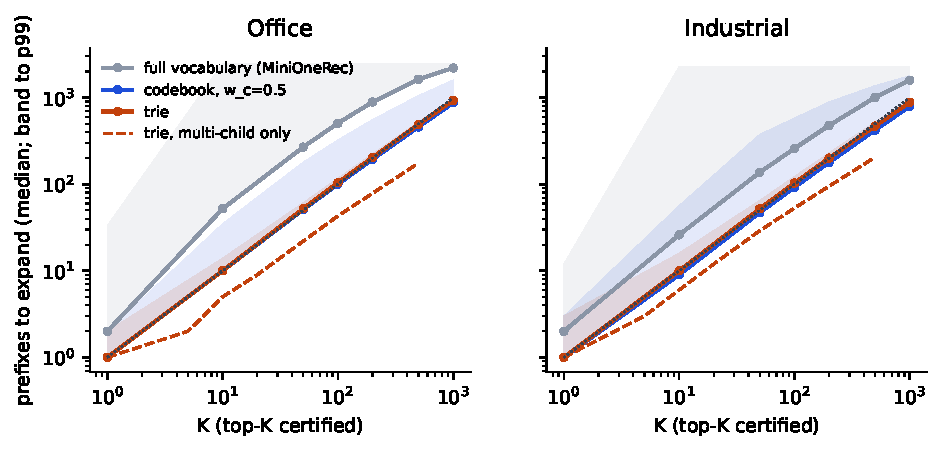
\includegraphics[width=0.78\linewidth]{certificate_kscale.pdf}
\caption{Prefixes the certificate must expand to prove the top $K$ (median; band to p99), from exhaustive FP32 scores of all test users. Under trie or codebook normalization the cost is about $K$ prefixes; under MiniOneRec's full-vocabulary objective it approaches the whole trie.}
\label{fig:kscale}
\end{figure}

{\small
\setlength{\tabcolsep}{4pt}
\begin{xltabular}{\linewidth}{>{\raggedright\arraybackslash\hsize=1.957\hsize}X>{\raggedright\arraybackslash\hsize=0.666\hsize}X>{\raggedright\arraybackslash\hsize=0.737\hsize}X>{\raggedright\arraybackslash\hsize=0.880\hsize}X>{\raggedright\arraybackslash\hsize=0.880\hsize}X>{\raggedright\arraybackslash\hsize=0.880\hsize}X}
\toprule
prefixes to expand (median / p90 / p99) & K=10 & K=50 & K=100 & K=500 & K=1000 \\
\midrule
\endhead
Office, trie & 10 / 12 / 14 & 52 / 57 / 61 & 104 / 111 / 117 & 489 / 510 / 524 & 932 / 960 / 979 \\
Office, codebook $w_{c}$=0.5 & 10 / 13 / 35 & 51 / 61 / 180 & 100 / 117 / 325 & 459 / 517 / 1,058 & 871 / 962 / 1,600 \\
Office, full vocabulary (MiniOneRec) & 52 / 1,715 / 2,488 & 268 / 2,462 / 2,488 & 506 / 2,486 / 2,488 & — & — \\
Industrial, trie & 10 / 13 / 16 & 52 / 60 / 65 & 103 / 115 / 123 & 470 / 501 / 522 & 881 / 922 / 948 \\
\bottomrule
\end{xltabular}
}

Under trie normalization the bound is almost tight: certifying the top K costs about K prefix expansions at every K, with a thin tail. Under the full-vocabulary objective the off-codebook leak and the suffix make $U_2$ loose and certification needs nearly the whole trie. The normalization choice therefore decides whether exact search is affordable at all.

Trie normalization gives a second saving. The third-code term is a log-softmax over the valid children of (a,b), so it is exactly 0 when (a,b) has one child: every item under a single-child prefix is exactly scored by the first forward. Only multi-child prefixes need the second forward (Office: 581 of 2,488 prefixes, holding 1,537 of 3,444 items):

{\small
\setlength{\tabcolsep}{4pt}
\begin{longtable}{lllll}
\toprule
multi-child prefixes to expand (median / p90 / p99) & K=10 & K=50 & K=100 & K=500 \\
\midrule
\endhead
Office, trie & 5 / 8 / 10 & 22 / 31 / 38 & 43 / 55 / 64 & 175 / 198 / 213 \\
Industrial, trie & 6 / 9 / 12 & 29 / 37 / 43 & 53 / 65 / 75 & 205 / 238 / 259 \\
\bottomrule
\end{longtable}
}

\code{ExactTrieEngine} expands only multi-child prefixes; its candidate pool is the expanded children plus every single-child item, both exact. It reproduces the three-stage engine rank-for-rank and score-for-score (FP32). A certified top-500 is still two forwards, the second carrying ≈210 rows; beam-500 needs four forwards of 500 rows each (three with trie scoring).

\textbf{One forward is not enough.} Two ways to drop the second forward fail:

\begin{itemize}
\item \emph{A user-independent third-code table} (per-item mean of s(c|ab) over validation users) keeps HR@10 within 0.9 pt but drops HR@1 from 0.098 to 0.050 (−4.8 pt [−5.5, −4.1]). Item identity explains 77\% of the variance of s(c|ab) overall but only 42\% within a user's top-50; the third code orders siblings per user.
\item \emph{Speculating the expansion set before the first forward} (from the user's previous request, history prefixes or popularity) covers the full certificate set for top-10 in at most 29\% of requests with 128 guessed prefixes; certification needs the near-boundary prefixes too.
\end{itemize}

Certification after the first forward alone happens for 44\% of users at K=1 and 0.5\% at K=10.

\subsection{Two-sided bounds: the expansion set is known after the first forward}\label{sec:5.1b}

Upper bounds alone say which prefixes \emph{might} hold a top-K item. Trie normalization also gives a \textbf{lower bound}: the third-code term is a log-softmax over the $n_{p}$ valid children of p = (a,b), so its largest child has log-prob ≥ −log $n_{p}$, and some item under p scores at least L(p) = U(p) − $w_{c}$ log $n_{p}$ (U(p) = s(a) + $w_{b}$ s(b|a), exact after forward 1). Single-child items are exactly scored by forward 1.

\begin{figure}[htp]
\centering
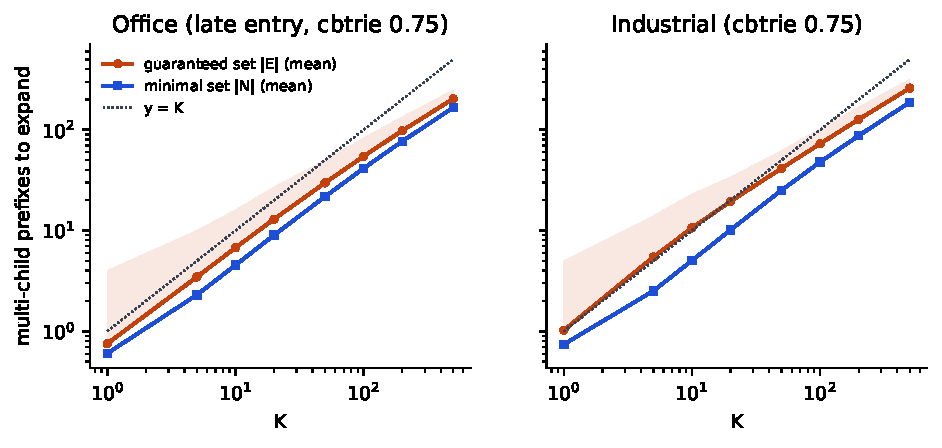
\includegraphics[width=0.78\linewidth]{two_sided_bounds.pdf}
\caption{The guaranteed expansion set $|E|$ (Prop.~3, known right after the first forward; band to p99) against the minimal set $|N|$ that any bound-based decoder must expand (Prop.~2); means over all test users.}
\label{fig:bounds}
\end{figure}

\begin{itemize}
\item \textbf{Prop. 1 (soundness; known).} If the K-th exact pool score ≥ U of every unexpanded prefix, the pool's top K is the global top K (all terms ≤ 0).~\cite{stahlberg2019,stahlberg2022,fagin2003}; stated for GR as post-hoc beam completion in \emph{Beyond the Beam}~\cite{ax2609.33745}.
\item \textbf{Prop. 2 (necessity / instance optimality).} Let τ\textsuperscript{*} be the true K-th score. Any algorithm whose only information about an unexpanded prefix is U(p) must expand every multi-child p with U(p) > τ\textsuperscript{*}: the children's log-softmax can put its mass on one child scoring U(p) − ε > τ\textsuperscript{*}, which would enter the top K. So N = \{p : U(p) > τ\textsuperscript{*}\} is a lower bound for every bound-based decoder, and best-first expansion by U reaches it (up to ties).
\item \textbf{Prop. 3 (guaranteed expansion set).} Let $τ_{L}$ be the K-th largest value of \{exact single-child scores\} ∪ \{L(p) : p multi-child\}. K distinct items score ≥ $τ_{L}$, so $τ_{L}$ ≤ τ\textsuperscript{*}. Expanding E = \{p multi-child : U(p) ≥ $τ_{L}$\} ⊇ N always certifies: the pool then contains those K items, and every unexpanded prefix has U < $τ_{L}$. |E| is computed on device right after forward 1; E $\setminus$ N contains only prefixes with $τ_{L}$ ≤ U < τ\textsuperscript{*}, a band of width ≤ τ\textsuperscript{*} − $τ_{L}$ ≤ $w_{c}$ log $n_{\max}$.
\item Codebook or full-vocabulary normalization of the last level admits no such lower bound (the valid children can hold arbitrarily little mass), so this is a property of trie normalization only.
\end{itemize}

Measured on all test users (\code{scripts/\allowbreak{}lbound.py}, \code{runs/\allowbreak{}lbndA}; |E| mean / p99 / max vs the minimal |N| mean / max):

{\small
\setlength{\tabcolsep}{4pt}
\begin{longtable}{llll}
\toprule
K & Office (cascade late entry, cbtrie 0.75) & Office (trie, full depth) & Industrial (cbtrie 0.75) \\
\midrule
\endhead
1 & 0.8 / 4 / 8 vs 0.6 / 3 & 0.8 / 4 / 13 vs 0.6 / 5 & 1.0 / 5 / 9 vs 0.7 / 4 \\
10 & 6.7 / 16 / 24 vs 4.5 / 13 & 7.0 / 18 / 26 vs 4.9 / 13 & 10.6 / 23 / 29 vs 5.0 / 14 \\
50 & 29.7 / 50 / 62 vs 21.7 / 43 & 30.4 / 53 / 62 vs 22.7 / 44 & 41.5 / 62 / 75 vs 25.1 / 45 \\
100 & 54.6 / 83 / 99 vs 41.5 / 71 & 55.7 / 86 / 101 vs 43.2 / 80 & 72.7 / 102 / 116 vs 47.9 / 81 \\
500 & 203 / 248 / 267 vs 166 / 220 & 206 / 255 / 276 vs 172 / 225 & 259 / 318 / 342 vs 188 / 256 \\
\bottomrule
\end{longtable}
}

The guaranteed set is ≤ 1.1 K prefixes on average at every K (0.41 K at K=500) and 1.2–2.1× the provable minimum. In serving terms: forward 2 is a fixed-shape graph with M rows; with M ≥ max |E| (Office top-10: 24) certification is guaranteed before forward 2 runs, and an overflow (|E| > M) is detected after forward 1 rather than discovered after forward 2. Our M=16 configuration covers |E| for 99\% of Office users and still certifies 100\% because E over-approximates N.

\subsection{Catalog scaling: the expansion the certificate needs does not grow with the catalog}\label{sec:5.1c}

The released catalogs are small (3,444 SIDs), but the model's vocabulary addresses 88 × 256 × 256 = 5.8M SIDs, so we densify the trie and run the real model on real prompts (\code{scripts/\allowbreak{}scale\_\allowbreak{}catalog.py}, 500 Office test users, cascade late entry, cbtrie 0.75). Quality is meaningless on synthetic items; cost and certification are not. \emph{siblings} adds third codes under the 2,488 real (a, b) prefixes (10k–300k SIDs, up to 145 children per prefix); \emph{prefixes} adds new (b, c) under the 88 real first codes, with codes drawn from the real per-level frequencies (10k–1M SIDs, up to 22,488 prefixes and 215 children). |N| is the minimal set any bound-based decoder must expand (Prop. 2), |E| the guaranteed set (Prop. 3); certification is that of the deployed engine at budget M.

{\footnotesize
\setlength{\tabcolsep}{4pt}
\begin{xltabular}{\linewidth}{>{\raggedright\arraybackslash\hsize=1.587\hsize}Xrr>{\raggedright\arraybackslash\hsize=0.937\hsize}Xr>{\raggedright\arraybackslash\hsize=0.863\hsize}X>{\raggedright\arraybackslash\hsize=0.863\hsize}X>{\raggedright\arraybackslash\hsize=0.750\hsize}X}
\toprule
catalog & SIDs & prefixes (max children) & |N| K=10 / 50 / 500 & |E| K=10 & top-10 cert. M=16 / 32 & top-50 cert. M=64 / 128 & A6000 ms, M=16 / 64 \\
\midrule
\endhead
real & 3,444 & 2,488 (12) & 4.7 / 22 / 167 & 7.3 & 100 / 100\% & 100 / 100\% & 6.33 / — \\
siblings & 100k & 2,488 (60) & 8.3 / 42 / 412 & 272 & 100 / 100\% & 99.6 / 100\% & 6.34 / 6.41 \\
siblings & 300k & 2,488 (145) & 8.4 / 41 / 396 & 537 & 99.8 / 100\% & 98.2 / 100\% & 6.34 / 6.42 \\
prefixes & 100k & 19,853 (45) & 8.4 / 45 / 417 & 48 & 100 / 100\% & 100 / 100\% & 6.35 / 6.41 \\
prefixes & 1M & 22,488 (215) & 8.4 / 41 / 411 & 290 & 99.6 / 100\% & 99.2 / 100\% & 6.36 / 6.40 \\
\bottomrule
\end{xltabular}
}

\begin{itemize}
\item \textbf{The minimal expansion is flat in catalog size}: |N| ≈ 8.4 / 42 / 410 for K = 10 / 50 / 500 from 10k to 1M SIDs (all sizes in \code{research/\allowbreak{}scale\_\allowbreak{}catalog\_\allowbreak{}office.json}). It is smaller on the real catalog only because 1,907 of its 2,488 prefixes have a single child and are exact after forward 1.
\item \textbf{So is the latency at a fixed budget}: in one allocation (\code{runs/\allowbreak{}scaleP}, 2×500 requests each) the real catalog takes 6.33 / 6.32 ms (run before and after) and the 1M-SID catalog 6.36 ms at M = 16 and 6.36 ms at M = 32 (+0.5\%); siblings-300k at M = 32 6.35 ms. Forward 1 carries the prompt and the 88 first-level rows whatever the catalog (the second code is a restricted LM head over ≤ 256 codes), forward 2 carries M rows, and the third-code head has ≤ 256 columns. Certified top-10 at M = 16 holds for ≥ 99.6\% of users at every size and at M = 32 for 100\%; top-50 needs M = 64 (≥ 98.2\%) or 128 (100\%); top-500 needs M ≥ 512 on the dense catalogs (|N| ≈ 410; 83–100\% certified at M = 512).
\item \textbf{Industrial replicates it} (48 first codes, cascade bridges at 18, \code{runs/\allowbreak{}scaleI}, A40, \code{research/\allowbreak{}scale\_\allowbreak{}catalog\_\allowbreak{}industrial.json}): |N| ≈ 7.8 / 38 / 350 for K = 10 / 50 / 500 from 10k to 1M SIDs (real: 5.2 / 25 / 186); certified top-10 ≥ 98.6\% at M = 16 and 100\% at M = 32, top-50 100\% at M = 128, at every size; latency at M = 16: real catalog 9.24 / 9.24 ms (before / after), 1M SIDs 9.32 ms (M = 32: 9.28 ms).
\item \textbf{The two-sided guarantee does not scale}: |E| grows with the number of children (K = 10: 7 → 290–537) because the −$w_{c}$ log n lower bound loosens. The certificate itself uses the forward-2 scores and is unaffected, so on dense tries size forward 2 by a fixed M (with a fallback for the rare uncertified request), not by E.
\item Caveat: synthetic items have no training signal of their own; the model scores them through their codes. A model trained on a 1M-item catalog may spread or sharpen its prefix distribution differently.
\end{itemize}

\begin{figure}[htp]
\centering
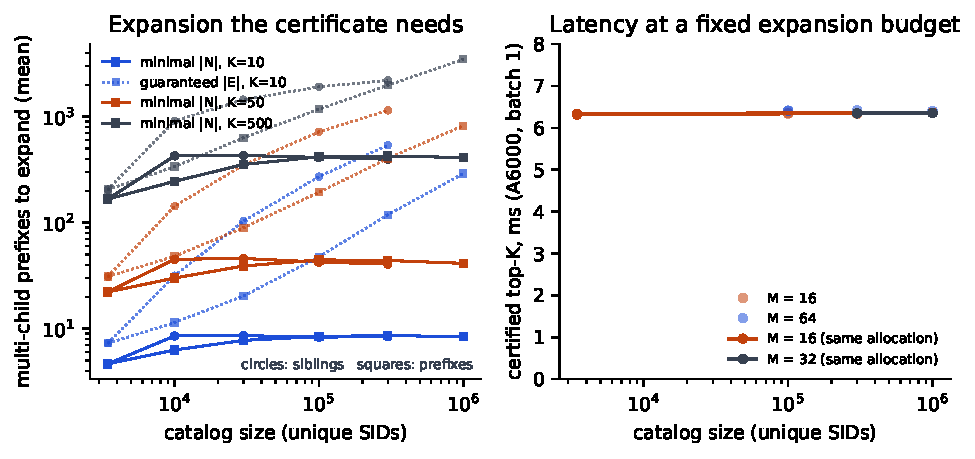
\includegraphics[width=0.90\linewidth]{catalog_scaling.pdf}
\caption{Synthetic catalogs of 10k--1M SIDs scored by the real model (500 Office test users). Left: the minimal expansion $|N|$ is flat in catalog size, while the guaranteed set $|E|$ grows with branching. Right: certified top-$K$ latency at a fixed budget $M$ (A6000, batch 1).}
\label{fig:catalog-scaling}
\end{figure}

\subsection{Late entry: the third code does not need the lower layers}\label{sec:5.2}

The logit lens shows SID codes are decided in the last 6–9 of 28 layers, and early exit (running only the \emph{first} k layers for the third code) keeps HR@10 but loses 2.4–3.7 points of HR@1. We instead let the prefix rows of the second forward \emph{enter late}: a row (a,b) starts at layer e with an input built from its parent node's residual stream at layer e — already computed for every first code in forward 1 — and runs layers e..27 with exact attention to the prompt and parent K/V. The input comes from a small bridge,

\begin{figure}[htp]
\centering
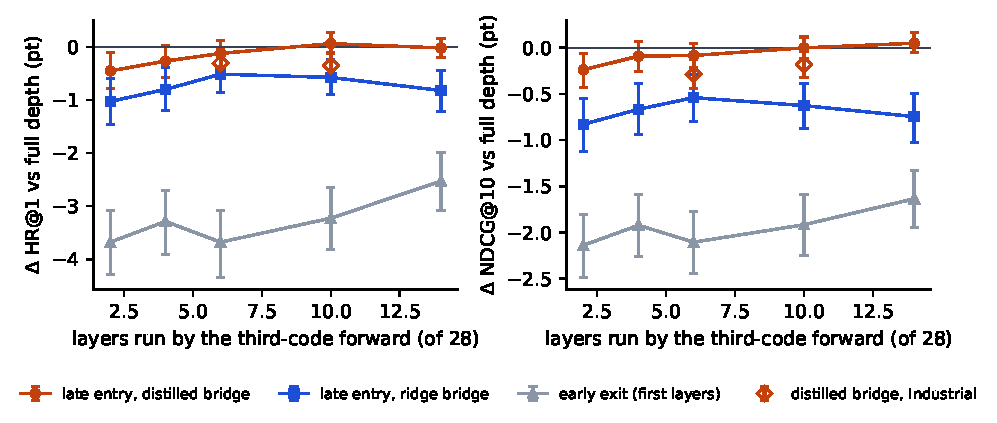
\includegraphics[width=0.90\linewidth]{late_entry_frontier.pdf}
\caption{Late entry against early exit for the third-code forward, paired against the full-depth forward (Office, all test users, 95\% bootstrap intervals). Bridged rows that enter at layer $28-k$ stay lossless down to 2--6 remaining layers; running only the first $k$ layers loses 2.5--3.7 points of HR@1.}
\label{fig:lateentry}
\end{figure}

\begin{equation}
x_e(a,b) = h_e(a) + R_e\,\bigl[h_e(a);\, E[b];\, E[a];\, 1\bigr]
  + \mathrm{MLP}_e\bigl(\bigl[\mathrm{rms}(h_e(a));\, E[b];\, E[a]\bigr]\bigr),
\label{eq:bridge}
\end{equation}

\noindent where $R_{e}$ is a ridge fit (label-free) and the MLP (2,048 hidden units, output zero-initialized) is distilled from the model itself: KL between the full-depth and the late-entry third-code distributions on MiniOneRec \emph{validation} prompts, weighting each prefix row half uniformly and half by the softmax of its bound $U_2$ (the rows that decide the ranking). Training takes 1–2 minutes on one H100; no item labels are used and the base model is frozen. The certificate holds for the late-entry objective. At serving time the bridge runs in FP16 (two small GEMMs).

All test users, validation-tuned codebook objective ($w_{c}$ = 0.5), FP16, paired against the full-depth third code (Office HR@1 0.0980 / HR@10 0.1706 / NDCG@10 0.1312; Industrial 0.0847 / 0.1613 / 0.1181):

{\footnotesize
\setlength{\tabcolsep}{4pt}
\begin{xltabular}{\linewidth}{>{\raggedright\arraybackslash\hsize=1.078\hsize}Xr>{\raggedright\arraybackslash\hsize=0.974\hsize}X>{\raggedright\arraybackslash\hsize=0.974\hsize}X>{\raggedright\arraybackslash\hsize=0.974\hsize}Xr}
\toprule
second forward & layers & ΔHR@1 & ΔHR@10 & ΔNDCG@10 & top-1 = full \\
\midrule
\endhead
Office, early exit (first k layers) & 6 & −3.68 [−4.34, −3.08] & −0.84 [−1.29, −0.39] & −2.11 [−2.44, −1.77] & 53\% \\
Office, late entry, ridge bridge & 6 & −0.51 [−0.86, −0.14] & −0.58 [−1.05, −0.14] & −0.54 [−0.80, −0.29] & 66\% \\
Office, late entry, distilled bridge (uniform KL) & 6 & −0.12 [−0.37, +0.12] & −0.12 [−0.35, +0.08] & −0.08 [−0.22, +0.04] & 92\% \\
\textbf{Office, late entry, distilled bridge (weighted KL)} & \textbf{6} & \textbf{+0.27 [+0.12, +0.45]} & \textbf{−0.04 [−0.25, +0.16]} & \textbf{+0.10 [−0.01, +0.20]} & \textbf{94\%} \\
Office, distilled bridge (uniform) & 2 / 4 / 10 / 14 & −0.45 / −0.27 / +0.06 / −0.02 & −0.09 / +0.04 / — / +0.14 & −0.24 / −0.09 / −0.00 / +0.05 & 86–94\% \\
Industrial, early exit & 10 & −2.38 [−2.96, −1.83] & −0.77 [−1.30, −0.20] & −1.80 [−2.18, −1.40] & 47\% \\
Industrial, distilled bridge (uniform KL) & 10 & −0.35 [−0.62, −0.11] & −0.04 [−0.31, +0.20] & −0.18 [−0.33, −0.04] & 86\% \\
\textbf{Industrial, distilled bridge (weighted KL)} & \textbf{10} & \textbf{−0.07 [−0.22, +0.09]} & \textbf{−0.04 [−0.24, +0.18]} & \textbf{−0.04 [−0.13, +0.05]} & \textbf{92\%} \\
\bottomrule
\end{xltabular}
}

With prefix-weighted distillation, late entry is statistically indistinguishable from the full-depth second forward on HR@10 and NDCG@10 on both datasets (Office at 6 remaining layers, Industrial at 10), and stays above the MiniOneRec reference decode (Office HR@10 0.1702 vs 0.1589). The small HR@1 gain on Office is a calibration side effect of the bridged objective, not a claim we rely on. Late entry of the \emph{second} code (the 88 first-code rows joining forward 1 at layer 22, bridged from the last prompt token) is a trade-off: ΔNDCG@10 −0.25 [−0.51, −0.01], and only 61\% of top-10 prefixes agree with full depth; the second code decides set membership.

Engine latency (CUDA graph, FP16, paired within one allocation; certified top-10):

{\small
\setlength{\tabcolsep}{4pt}
\begin{longtable}{lrr}
\toprule
 & A6000 & H100 \\
\midrule
\endhead
certified exact, trie, M=16 & 13.65 & 5.03–5.47 \\
+ Triton prompt attention in forward 1 & 13.26 & 4.56 \\
+ late entry at layer 22 & \textbf{9.06} & 3.56 \\
+ whole-layer compile, FP16 bridge & 9.07 & \textbf{3.24} \\
certified exact, tuned codebook, M=64 → + late entry 22 & 14.33 → 9.68 & 5.57 → 4.17 \\
certified top-500 → + late entry + fast forward 1 & 17.95 → 10.09 & 6.06 → 3.36 \\
\bottomrule
\end{longtable}
}

Industrial \& Scientific (all 4,533 test users; paired against our fastest FP16 engine running MiniOneRec's own beam-50 on the same GPU): MiniOneRec beam 25.75 ms (A6000) / 8.37 ms (H100), HR@10 0.1582; certified trie 12.89 / 4.23 ms, HR@10 0.1588; \textbf{+ late entry at layer 18: 9.40 / 3.22 ms, HR@10 0.1597} (ΔHR@10 +0.18 [−0.38, +0.71], ΔNDCG@10 −0.08 [−0.36, +0.20], ΔHR@1 −0.29 [−0.64, +0.07]) — quality-neutral at 2.7× / 2.6× the speed.

\subsection{Other backbones: 3B and 7B, and an RL-tuned checkpoint}\label{sec:5.3}

Everything above uses the released 1.5B checkpoint. Public MiniOneRec-format checkpoints let us test the method on other backbones without training them ourselves (all H100, batch 1, all test users, paired against each model's own baselines):

\begin{itemize}
\item \textbf{Qwen2.5-3B and -7B} SFT with MiniOneRec's script on Office (HF \code{acdxuan/\allowbreak{}minionerec}), with the \emph{same} 600 SID tokens, catalog and test split as the release. Both are weaker than the released 1.5B under beam-50 (HR@10 0.1488 and 0.1443 vs 0.1587); we evaluate the decoder, not the checkpoints. The 7B has 4 KV heads, so the Triton attention kernels were generalized to any group size.
\item \textbf{An SFT / RL pair} on Industrial with its own RQ-VAE index (HF \code{onesfour/\allowbreak{}MiniOneRec-{}1.5B-{}SFT-{}GDPO}; GDPO is a GRPO variant trained with constrained beam-search rollouts). Its index gives 19\% of items a fourth code that separates collisions; our 3-level decoder merges each of the 268 collision groups into one SID, so both decoders below are evaluated on 3-code groups under trie normalization without the forced suffix.
\end{itemize}

{\footnotesize
\setlength{\tabcolsep}{4pt}
\begin{xltabular}{\linewidth}{>{\raggedright\arraybackslash\hsize=0.517\hsize}Xr>{\raggedright\arraybackslash\hsize=1.092\hsize}X>{\raggedright\arraybackslash\hsize=1.312\hsize}X>{\raggedright\arraybackslash\hsize=1.079\hsize}X}
\toprule
backbone & beam-50 ms & certified, full depth ms (ΔHR@10 vs beam) & + bridges ms (ΔHR@10 vs full depth) & + SASRec in the graph: ms, HR@10 (Δ) \\
\midrule
\endhead
1.5B (release) & 8.43 & 4.35 (+0.90 HR@10 vs beam) & 2.75, both bridges (+0.12 [−0.27, +0.51]) & 2.89, 0.1825 (+1.11) \\
3B (36 layers) & 13.01 & 6.91 (+0.12 [−0.18, +0.43]); top-10 cert. 100\% & 4.70, third code at 28 (−0.06 [−0.31, +0.18]) & 5.03, \textbf{0.1716 (+2.22 [+1.64, +2.79])} \\
7B (28 layers) & 21.07 & 11.74 (+0.04 [−0.25, +0.33]); 99.96\% & 7.78, third code at 22 (−0.02 [−0.18, +0.14]); both bridges 7.56 (−0.25 [−0.60, +0.08]) & 8.00, \textbf{0.1683 (+2.38 [+1.81, +2.96])} \\
1.5B SFT (Industrial, own index) & 5.81 & 4.67 (+0.02 [−0.04, +0.09]); 100\% & — & — \\
1.5B GDPO (RL) & 5.81 & 5.02 (−0.02 [−0.07, 0.00]); 100\% & — & — \\
\bottomrule
\end{xltabular}
}

\begin{itemize}
\item \textbf{Certification and the 1.8–1.9× full-depth speedup carry over unchanged} to a deeper (36-layer) and a wider (7B) model; certified top-10 is 99.8–100\% everywhere. With the third-code bridge the 3B and 7B decode in 4.70 and 7.78 ms, 2.8× and 2.7× faster than their own beam-50 at equal quality (beam re-timed in the same allocations: 13.01 and 21.05 ms). FP8 + fusion throughput: 955 (3B) and 467 (7B) users/s at B = 32, quality-neutral (HR@10 0.1702, 0.1679).
\item \textbf{Late entry transfers with the same recipe} (entry layers scaled by depth, 3 epochs, validation prompts only): the third-code bridge is lossless on both; the first-level bridge is ≈lossless on 7B (−0.18 [−0.49, +0.08]) but not on 3B at layer 23 of 36 (−0.37 [−0.74, −0.02]), where it would save only 0.16 ms — choose entries on validation per model, as for the fine-tuned 1.5B (\S\ref{sec:6.y}).
\item \textbf{Fusion helps more when the LLM is weaker}: the same SASRec term and β add +2.22 / +2.38 HR@10 and +3.49 / +3.43 HR@50 to the 3B / 7B (vs +1.11 / +2.08 on the 1.5B), lifting both above the released 1.5B LLM alone.
\item \textbf{RL sharpens the distribution and makes certification cheaper}, but does not change beam's search error under trie scoring: top-50 is certified at M = 16 for 26–31\% of users with GDPO vs 14–20\% with SFT; beam-50 and exact return the same top-10 set for 95–96\% of users on both. Under this (merged-collision, trie) evaluation GDPO trails its SFT parent by 1.96 [1.19, 2.71] HR@10; GDPO was optimized for full-vocabulary 4-code beam decoding, so this is a decoding-objective mismatch, not a verdict on RL.
\end{itemize}

\section{What exact decoding reveals about the objective}\label{sec:6}

\textbf{Beam search error is real but is not what limits quality.} From exhaustive FP32 scores of every catalog SID for every test user (\code{scripts/\allowbreak{}dump\_\allowbreak{}scores.py}), beam-50 under MiniOneRec's full-vocabulary objective recovers 86\% of the exact top-10 (top-1 exact for 99.8\% of users), yet exhaustive search gives the same HR@10. Under codebook or trie normalization beam-50 is essentially exact (99.6\% / 99.9\% of the exact top-10).

\begin{figure}[htp]
\centering
\begin{minipage}[b]{0.54\linewidth}\centering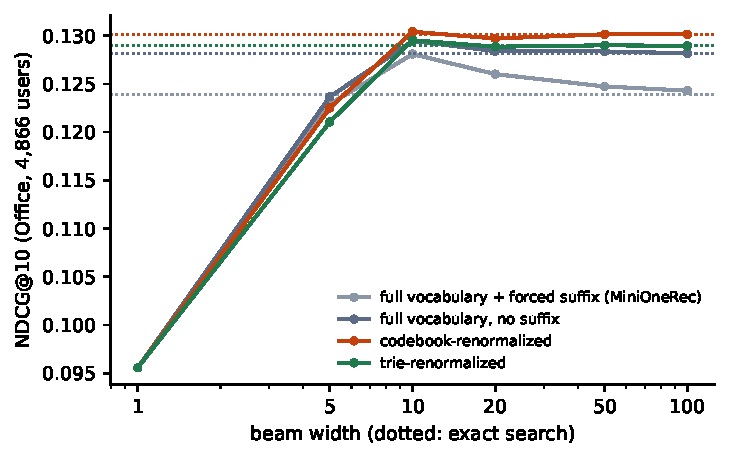
\includegraphics[width=\linewidth]{search_scoring_office.pdf}\end{minipage}\hfill
\begin{minipage}[b]{0.42\linewidth}\centering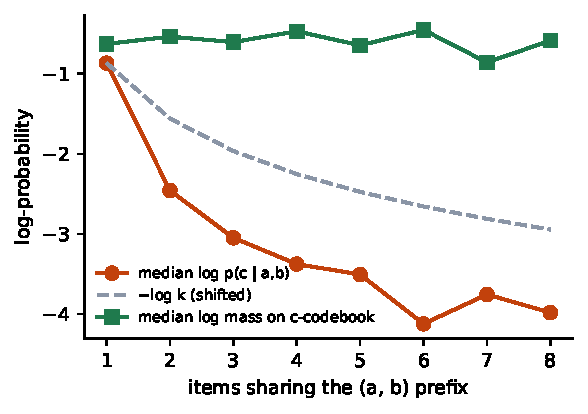
\includegraphics[width=\linewidth]{sibling_penalty_office.pdf}\end{minipage}
\caption{Left: NDCG@10 against beam width for four scoring rules (Office, all test users; dotted: exact search under the same rule). Right: the sibling penalty. The target's median $\log p(c \mid a,b)$ falls with the number of catalog items that share $(a,b)$, faster than an even split ($-\log k$), while the mass on the $c$-codebook stays flat (exhaustive FP32 scores).}
\label{fig:sibling_penalty_office}
\end{figure}

\textbf{The beam-search curse grows with list length.} Generative retrieval feeds hundreds of candidates to a ranker, so lists longer than 10 matter. Beam-W recovers only part of the exact top-W under the full objective (Office 49\% at W=50, 53\% at 100, 64\% at 500; Industrial 67 / 69 / 79\%); under trie scoring 95 / 96 / 99.6\%. Under the full objective, exact search \emph{loses} recall and the loss grows with K (Office, paired bootstrap vs MiniOneRec's beam-W decode): HR@50 −1.8 pt [−2.5, −1.1], HR@100 −2.5 [−3.3, −1.7], HR@200 −3.5 [−4.4, −2.5], HR@500 −4.3 [−5.3, −3.2]; Industrial −0.1 to −0.7 (n.s.). With the validation-tuned codebook objective exact search \emph{gains} recall on both datasets: Office HR@100 +2.3 [+1.5, +3.0], HR@500 +2.4 [+1.4, +3.3]; Industrial HR@200 +0.9 [+0.1, +1.6], HR@500 +0.9 [+0.0, +1.8]. Beam search's prefix-first pruning acts as an implicit depth discount; once the discount is explicit, exactness stops hurting.

\textbf{The objective is mis-calibrated in its deep terms.} Three independent signals:

\begin{enumerate}
\item Admitting fewer candidates by prefix bound improves HR@10 (N=16: +0.70 pt [+0.12, +1.29] vs the FP32 reference); admitting more converges back to beam.
\item Dropping the forced newline/EOS terms improves NDCG@10 by +0.36 pt [+0.13, +0.61].
\item Restricted normalizations — what production engines do for speed — score better than the training objective (beam-50, full test set):
\end{enumerate}

{\small
\setlength{\tabcolsep}{4pt}
\begin{longtable}{lrrrr}
\toprule
scoring rule & HR@1 & HR@10 & NDCG@10 & HR@50 \\
\midrule
\endhead
full vocabulary, with forced suffix (MiniOneRec) & 0.0947 & 0.1589 & 0.1249 & 0.2370 \\
full vocabulary, no suffix & 0.0986 & 0.1624 & 0.1284 & 0.2363 \\
trie-renormalized & 0.0982 & 0.1648 & 0.1287 & 0.2417 \\
codebook-renormalized (FlashRec-style) & 0.0986 & 0.1667 & 0.1299 & 0.2470 \\
\bottomrule
\end{longtable}
}

\textbf{Depth-discounted scoring.} Weighting later SID levels less, score = lp(a) + $w_{b}$ lp(b|a) + $w_{c}$ lp(c|ab) + $w_{s}$(lp(\nl{})+lp(EOS)), is a two/three-parameter decode-time calibration that keeps every term ≤ 0, so certified exact decoding applies unchanged. In-sample on a quarter of the Office test users, w = (0.75, 0.3, 0.3) raises HR@10 by \ensuremath{\sim}10\% relative. Weights are tuned on MiniOneRec's validation split (grid, max NDCG@10, exhaustive scores) and evaluated once on test (\code{scripts/\allowbreak{}tune\_\allowbreak{}weights.py}): on Office this selects a discounted third code ($w_{c}$ = 0.5–0.75, +1.0–1.2 HR@10 over the reference decode); on Industrial no rule beats the original objective significantly (tuned codebook +0.35 [−0.26, +0.97]), so the scoring rule must be chosen per dataset. Why the deep terms mislead (exhaustive FP32 scores, 1,217 Office users × 3,444 SIDs):

\begin{itemize}
\item \textbf{Sibling penalty.} lp(c|ab) falls with the number of catalog items sharing the prefix (a,b): median −0.87, −2.46, −3.05, −3.38, −4.12 for 1, 2, 3, 4, 6 siblings (Pearson r = −0.36 between lp(c|ab) and sibling count over each user's top-50) — steeper than the −log k of an even split (−1.6 nats from one to two siblings vs log 2 = 0.69). This is a structural penalty on items that share a prefix, unrelated to the user (Fig. \ref{fig:sibling_penalty_office}).
\item \textbf{Codebook leakage.} Even after a valid (a,b), a median 47\% of next-token mass falls outside the c-codebook (median log-mass −0.63, flat across sibling counts); full-vocabulary scoring charges every item for it, unevenly across users and prefixes. Codebook/trie renormalization removes it.
\item \textbf{The forced suffix is mixed evidence.} On average the target's lp(\nl{})+lp(EOS) is higher than its competitors' (−1.69 vs −6.31; competitor mean dominated by a few very unlikely completions), but adding the suffix moves the target up for 28\% of users and down for 25\%; it correlates with log item popularity (r = 0.15) — a weak popularity prior that costs a forward.
\end{itemize}

These are consistent with SID-MLP's observation that SID difficulty concentrates in the first code: preference information lives in lp(a) and lp(b|a), while deeper terms are dominated by catalog structure.

\subsection{Exact search under value-augmented objectives}\label{sec:6.x}

Production rankers rarely serve the model's log-probability alone: they add item-level terms (priors, bids, freshness, a collaborative model's opinion). With beam search such a term can only be applied after the beam has pruned. Certified search handles any additive item term $v_{u}$(i) exactly: the bound of prefix p becomes $U(p) + \max_{i \text{ under } p} v_u(i)$ (a scatter-max per request), the expansion is still one forward of M rows, and the certificate is unchanged (\code{set\_\allowbreak{}item\_\allowbreak{}bonus}; per-user terms are read from a device buffer inside the CUDA graph).

\begin{figure}[htp]
\centering
\begin{minipage}[b]{0.36\linewidth}\centering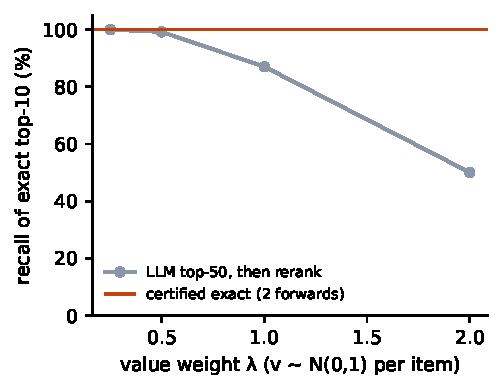
\includegraphics[width=\linewidth]{value_search_error.pdf}\end{minipage}\hfill
\begin{minipage}[b]{0.62\linewidth}\centering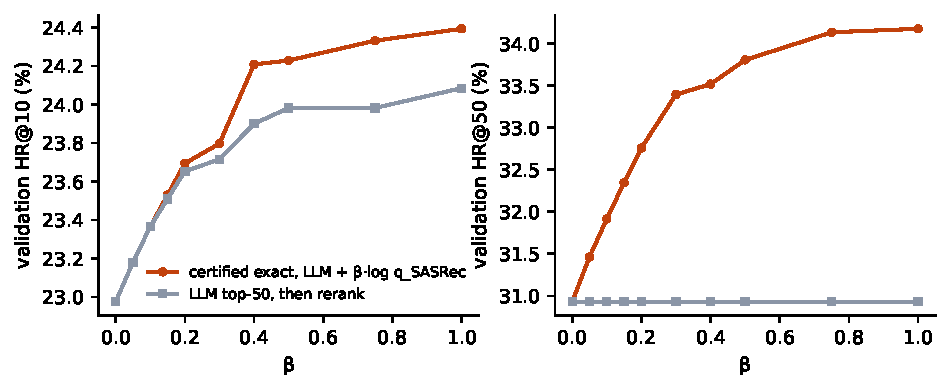
\includegraphics[width=\linewidth]{fusion_office.pdf}\end{minipage}
\caption{Left: recall of the exact top-10 under a synthetic per-item value term $\lambda v$, $v\sim\mathcal{N}(0,1)$. Reranking the LLM's top-50 degrades as $\lambda$ grows; certified search stays exact. Right: validation HR@10 and HR@50 against the SASRec weight $\beta$ (Office). Reranking cannot change the top-50 set, so its HR@50 is flat.}
\label{fig:fusion}
\end{figure}

\emph{Search error of beam-then-rerank.} With a synthetic per-item value v \ensuremath{\sim} N(0,1) weighted by λ, ``LLM top-50 then rerank'' (an upper bound on any beam-50 + rerank pipeline) recovers 99.99 / 99.2 / 87.0 / \textbf{50.0\%} of the exact top-10 at λ = 0.25 / 0.5 / 1 / 2 (Office, 2,000 users); certified search stays 100\% certified at M = 32.

\emph{Filters.} A filter (inventory, region, policy) is an item term of 0 or −∞; a prefix whose items are all excluded gets bound −∞ and is never expanded. Certified search returns the exact top-K \emph{eligible} items in the same two forwards and certified 100\% of users under every filter we tried. Filtering the LLM's own top-50 afterwards recovers 99.6 / 92.8 / \textbf{30.5\%} of the exact filtered top-10 at 50 / 20 / 5\% random eligibility (3 items survive at 5\%), and 88.3 / 68.0\% when only 25 / 10\% of first codes are allowed; HR@10 at 5\% eligibility drops from 0.029 to 0.018. Filtering a top-500 list recovers ≈99.7\% (residual: FP16 near-ties across batch shapes) — i.e. filter-after-retrieval needs a \ensuremath{\sim}10× longer candidate list to match two certified forwards (Office, 2,000 users, \code{runs/\allowbreak{}filtS}).

\emph{Collaborative fusion.} A SASRec~\cite{kang2018} (2 layers, d = 64, train split, 58 s on one GPU; alone: test HR@10 0.1500, NDCG@10 0.1156) supplies $v_{u}$(i) = β log q(i | history). β is chosen on validation (0.5). Office test, all 4,866 users:

{\small
\setlength{\tabcolsep}{4pt}
\begin{longtable}{lrrrr}
\toprule
decoder (Office test) & HR@1 & HR@10 & NDCG@10 & HR@50 \\
\midrule
\endhead
LLM, certified (cbtrie 0.75, both bridges) & 0.0993 & 0.1714 & 0.1319 & 0.2513 \\
LLM top-50, then rerank with β log q (β = 0.5) & 0.1021 & 0.1800 & 0.1377 & 0.2513 \\
\textbf{certified exact, LLM + β log q} & \textbf{0.1025} & \textbf{0.1825} & \textbf{0.1391} & \textbf{0.2721} \\
\bottomrule
\end{longtable}
}

vs the LLM alone: ΔHR@10 +1.11 [+0.62, +1.60], ΔNDCG@10 +0.72 [+0.45, +1.00], ΔHR@50 +2.08 [+1.44, +2.69]; vs rerank: ΔHR@10 +0.25 [+0.08, +0.43], ΔNDCG@10 +0.13 [+0.04, +0.23]. Against MiniOneRec's FP32 beam decode of the same checkpoint (0.1589) this is +2.36 points of HR@10 with no LLM training — on par with the best \emph{trained} result we found on the same split (DASO~\cite{ax2608.20611}, 0.1834) and above S-GRec~\cite{ax2602.10606}, V-STAR~\cite{ax2602.10699} and SA-OPSD~\cite{ax2611.01568} (0.1689–0.1747). Industrial (\code{runs/\allowbreak{}fuseI}, β = 0.5): HR@10 0.1617 → 0.1668 (+0.51 [+0.07, +0.95]), NDCG@10 +0.42 [+0.19, +0.66], HR@50 +0.84 [+0.22, +1.48]. At large K the fused certified top-500 lifts HR@500 by 4.0 points on Office (0.504 → 0.543) and 2.1 on Industrial (0.523 → 0.544), where reranking the LLM's own top 500 cannot change the set; Industrial top-500 certifies for 83–85\% of users at M = 256 under the fused objective and for 100\% at M = 512 (4.23 vs 3.50 ms, \code{runs/\allowbreak{}collabI}; Office: 100\% at M = 256). End to end, with SASRec computed inside the graph on a side stream from the user's 20-item history, the fused decoder takes 2.89 ms on Office (2.66 ms with precomputed SASRec rows, same allocation) and 3.09 ms on Industrial (3.07 ms), at identical quality; FP8 throughput with in-graph SASRec is 3,048 / 3,134 (Office) and 3,581 / 3,660 (Industrial) users/s at B = 64 / 128. (A \code{torch.compile}d SASRec head was faster but returned wrong values inside the graph; not used.)

\subsection{Training the model the decoder sees}\label{sec:6.y}

MiniOneRec is trained with full-vocabulary next-token cross-entropy, but our decoder ranks with per-level log-softmax over restricted sets (codebook for the first two codes, valid trie children for the third). We fine-tune the released checkpoint for one epoch on its own train split (38.9k rows, lr 1e-5, AdamW, bf16 autocast, one A40, 17.5 min) with exactly that restricted per-level cross-entropy on the three SID positions (\code{scripts/\allowbreak{}train\_\allowbreak{}sft.py}). Same certified decoder, full depth, all test users:

{\small
\setlength{\tabcolsep}{4pt}
\begin{longtable}{lrrrr}
\toprule
Office test (certified, cbtrie 0.75, full depth) & HR@1 & HR@10 & NDCG@10 & HR@50 \\
\midrule
\endhead
released checkpoint & 0.0988 & 0.1677 & 0.1304 & 0.2446 \\
+ 1 epoch, decoder-aligned restricted CE & 0.0991 & 0.1767 & 0.1345 & 0.2643 \\
+ 1 epoch, full-vocabulary CE (control) & 0.0978 & 0.1753 & 0.1337 & 0.2643 \\
aligned fine-tune + SASRec term (β = 0.3) & 0.1011 & \textbf{0.1852} & 0.1388 & 0.2797 \\
\bottomrule
\end{longtable}
}

Aligned vs released: ΔHR@10 +0.90 [+0.27, +1.54], ΔNDCG@10 +0.41 [+0.04, +0.78], ΔHR@50 +1.97 [+1.15, +2.77] (validation ΔHR@10 +1.27). \textbf{But the control gets almost all of it:} aligned vs full-vocabulary CE ΔHR@10 +0.14 [−0.16, +0.47], ΔNDCG@10 +0.08 [−0.07, +0.24], ΔHR@50 0.00 (validation ΔHR@10 −0.14). One more SFT epoch helps the released checkpoint; matching the training normalization to the decoder's does not measurably add to it — a negative result for the ``align training with decoding'' hypothesis. Bridges trained on the released model transfer imperfectly (entry 22: HR@10 0.1743), so a fine-tuned backbone needs its own bridges (\ensuremath{\sim}25 min). [Industrial replication and a second seed: Industrial ΔHR@10 +0.49 [−0.15, +1.13] (n.s.), ΔHR@50 +1.81 [+0.95, +2.65]; a second Office seed reproduces ΔHR@10 +0.86 [+0.21, +1.54].]

\section{Precision and quantization}\label{sec:7}

{\small
\setlength{\tabcolsep}{4pt}
\begin{xltabular}{\linewidth}{>{\raggedright\arraybackslash\hsize=1.000\hsize}Xrrrrr}
\toprule
precision (fused + Triton beam, full semantics) & ms & top-1 = FP32 & top-10 set = FP32 & identical 50-lists & max |Δscore| \\
\midrule
\endhead
FP32 (TF32 off) & 98.8–105.0 & 500/500 & 500/500 & — & — \\
FP16 (Q pre-scaled) & 27.5 & 500/500 & 484/500 & 151/500 & 0.15 \\
BF16 & 27.9 & 488/500 & 374/500 & 0/500 & 1.48 \\
\bottomrule
\end{xltabular}
}

FP16 is as fast as BF16 and \ensuremath{\sim}10× more faithful; HR/NDCG are statistically indistinguishable from FP32 for both. Weight-only INT8 (GemLite) is quality-neutral but only 3–8\% faster; INT4 (RTN, group 128) is no faster and less faithful. The kernel profile explains why: after fusion, GEMMs are ≈80\% of GPU time at ≈75\% of peak bandwidth, with M = 50–216 rows per forward — outside the M ≤ 16 regime where weight-only kernels shine. The roofline makes this explicit: one A6000 forward costs 8.1 / 9.8 / 12.2 / 16.1 ms at 1 / 50 / 128 / 256 tokens in BF16, versus 5.2 / 8.3 / 11.8 / 18.1 ms with INT8 weights. On an L40S, dynamic per-token FP8 W8A8 (\code{torch.\_\allowbreak{}scaled\_\allowbreak{}mm}, rowwise scales) is \emph{slower} than BF16 end to end (certified exact 15.9 vs 14.0 ms; beam 23.5 vs 20.1 ms) at near-equal quality, because quantizing activations at every GEMM outweighs the narrower weights at 50–216 rows; a quantize-in-RMSNorm FP8 path is future work.

\section{Throughput}\label{sec:8}

Users per second on one A6000 (BF16/FP16, cached template), batch B users per graph replay:

\begin{figure}[htp]
\centering
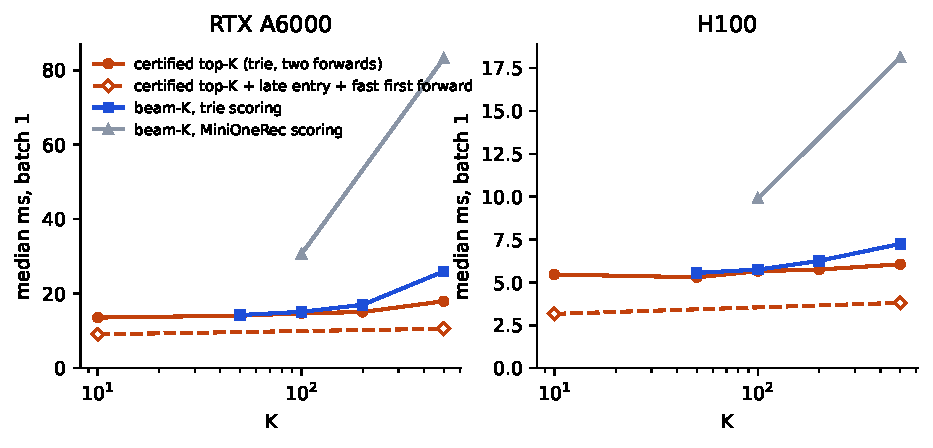
\includegraphics[width=0.72\linewidth]{large_k_latency.pdf}
\caption{Batch-1 latency against list length $K$. Certified top-$K$ stays nearly flat up to $K=500$; beam-$K$ does not, least of all under MiniOneRec's full-vocabulary scoring.}
\label{fig:largek}
\end{figure}

{\small
\setlength{\tabcolsep}{4pt}
\begin{longtable}{lrrrrr}
\toprule
decoder & B=1 & B=4 & B=8 & B=16 & B=32 \\
\midrule
\endhead
beam-50, full MiniOneRec scoring & 37.5 & 69.2 & 77.0 & 86.0 & 91.3 \\
certified exact, trie scoring & 67.8 & 135.6 & 145.9 & 165.2 & 172.2 \\
certified exact, tuned codebook & 67.8 & — & 160.5 & — & 176.2 \\
\bottomrule
\end{longtable}
}

Exact decoding processes fewer tokens per user (prompt tail + 88 trie nodes + 64 prefix rows vs prompt + 88 + 50 + 100 beam rows) and stays ≈1.9× ahead once both are compute-bound.

H100 (\code{runs/\allowbreak{}h100M}, \code{runs/\allowbreak{}largeKH}, \code{runs/\allowbreak{}tpK}, \code{runs/\allowbreak{}lateLH}), users/s:

{\small
\setlength{\tabcolsep}{4pt}
\begin{longtable}{lrrrr}
\toprule
decoder & B=1 & B=8 & B=32 & B=64 \\
\midrule
\endhead
certified exact, tuned codebook (M=64) & 178 & 726 & 904 & 920 \\
certified exact, trie, multi-child prefixes only (M=16) & 182 & 837 & 1,223 & — \\
+ late entry at layer 22 & 261 & 983 & 1,355 & 1,369 \\
\bottomrule
\end{longtable}
}

Large candidate lists (H100, users/s): certified top-500 173 / 374 / 414 / 450 at B = 1/4/8/16; beam-500 with trie scoring 132 / 229 / 253 (B = 1/4/8); MiniOneRec's beam-500 (full vocabulary, forced suffix) 54 / 68 / 71 — \textbf{6.4×} at the largest batch each fits. Certified top-100: 185 / 689 / 858 (B = 1/8/32) vs trie beam-100 169 / 628 / 740.

\subsection{Against a public SID-GR engine on the same GPU}\label{sec:8.1}

We compare with FlashRec 0.1.2~\cite{flashrec} (sohu-mptc/FlashRec @ 1089682, Apache-2.0), the open-source engine built for this workload: CUDA-graph wide beam including the expansion step, a fused CUDA trie kernel, a restricted per-codebook LM head, a radix prefix cache and cross-request decode waves, FP8 by default. NVIDIA's SID-GR example~\cite{nvidiasidgr} could not be run as published: its decode-attention kernel is a private submodule (\code{gr-{}decode-{}attention}; the repository it points to and the fork named in its README return 404), so outside users get only a placeholder backend. FlashRec supports Qwen3 only; a 60-line patch (\code{scripts/\allowbreak{}flashrec\_\allowbreak{}qwen2.py}) adds Qwen2 (QKV bias, no QK-norm). It decodes our exact prompt token ids and catalog (3,444 SIDs, beam 50, 3 steps) with its own CUDA graphs (captured at 19 sizes) and JIT trie kernel (verified loaded). Its radix cache holds our 69-token shared prefix (the counterpart of our template cache) and every other prefix is evicted before each timed request. FlashRec latency is the wall time of its offline API, \code{engine.generate()}, from token ids to ranked beams on the host; ours is a pinned host prompt through one graph replay (+ the copy of the ranked list to the host). One H100 allocation per table (\code{runs/\allowbreak{}frLat}, \code{runs/\allowbreak{}frTp}; \code{scripts/\allowbreak{}flashrec\_\allowbreak{}job.sh}, \code{scripts/\allowbreak{}compare\_\allowbreak{}flashrec.py}).

{\small
\setlength{\tabcolsep}{4pt}
\begin{xltabular}{\linewidth}{>{\raggedright\arraybackslash\hsize=1.000\hsize}Xrrr}
\toprule
engine / decoder (H100, batch 1) & median ms & p95 & HR@10, all 4,866 users \\
\midrule
\endhead
FlashRec BF16 & 11.48 & 11.64 & 0.1644 \\
FlashRec FP16 & 11.71 & 12.02 & 0.1644 \\
FlashRec FP8 (its default) & 14.22 & 14.45 & 0.1554 \\
ours, beam-50 under FlashRec's objective (per-level codebook softmax, no suffix) & 5.15 (5.19) & 5.30 & 0.1679 \\
ours, beam-50, MiniOneRec semantics & 8.36 (8.39) & 9.04 & 0.1587 \\
ours, certified, late entry 18 / 26 & \textbf{2.57} (2.59) & 2.65 & 0.1689† \\
ours, certified + SASRec term computed in the graph & \textbf{2.83} (2.85) & 2.92 & \textbf{0.1825}† \\
\bottomrule
\end{xltabular}
}

Parentheses: with the device-to-host copy. †Quality of the same configurations from earlier runs (\code{runs/\allowbreak{}e26H}, \code{runs/\allowbreak{}collabO}); beam-50 MiniOneRec semantics from \code{runs/\allowbreak{}finalH}.

{\small
\setlength{\tabcolsep}{4pt}
\begin{longtable}{ll}
\toprule
users/s (H100), B = 16 / 32 / 64 / 128 &  \\
\midrule
\endhead
FlashRec FP16 & 408 / 431 / 428 / 500 \\
FlashRec FP8 & 433 / 370 / 363 / 489 \\
ours, beam-50 & 457 / 478 / 489 / — \\
ours, certified, FP16 & \textbf{2,310 / 2,559 / 2,678 / 2,681} \\
ours, certified, dynamic FP8 & \textbf{2,391 / 2,896 / 3,077 / 3,148} \\
\bottomrule
\end{longtable}
}

\begin{figure}[htp]
\centering
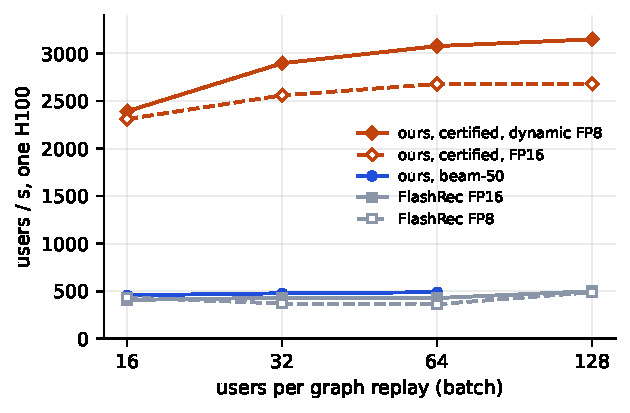
\includegraphics[width=0.60\linewidth]{flashrec_throughput.pdf}
\caption{Throughput on one H100 against batch size (\code{runs/frTp}). With beam-50 both engines serve the same number of users per second; certified decoding serves 5.4--6.4$\times$ more.}
\label{fig:flashrec-tp}
\end{figure}

\begin{itemize}
\item \textbf{4.5× lower latency and 5.4–6.4× higher throughput.} The gap is not an artifact of the timing boundary: FlashRec's CUDA-kernel time alone is 6.78 ms per request (1,878 kernels; profiler over 50 requests), more than our end-to-end 2.57 ms; the rest of its 11.7 ms is host-side scheduling.
\item \textbf{The engines are comparable; the decoder is not.} Running beam-50, our engine and FlashRec reach the same throughput (457–489 vs 408–500 users/s); the 5–6× comes from certified decoding processing fewer tokens per user. At batch 1 our beam-50 under FlashRec's own objective is 2.3× faster than FlashRec.
\item \textbf{FP8 does not pay at batch 1 on this checkpoint}: FlashRec's default is slower than BF16 (14.2 vs 11.5 ms) and loses 0.90 HR@10 [−1.32, −0.47] against its own FP16.
\item \textbf{Quality.} Paired against FlashRec FP16: our exact beam under its objective +0.35 HR@10 [+0.04, +0.64], certified (late entry 18/26) +0.45 [+0.00, +0.90], certified with both bridges at 18/22 +0.68 [+0.25, +1.15], fused +1.81 [+1.23, +2.36]. Part of FlashRec's deficit is numerical: on our Qwen2 port its first-code log-probabilities differ from the Hugging Face FP32 model by 0.23 nats on average (half-precision HF: 0.002 in FP16, 0.02 in BF16), and its top-1 agrees with exact beam under the same objective for 80\% of users. We could not attribute this to its prefix cache, CUDA graphs, fused expansion, per-codebook head, GQA grouping (a 12-KV-head copy of the checkpoint drifts the same), output-layer tying or Q/K layout; widening its per-beam candidate cut from 2×beam to the full codebook changes nothing. We therefore take our exact implementation of its objective (0.1679) as the quality FlashRec's design would reach: certified decoding matches it (+0.10 [−0.31, +0.58]) at half the latency of that beam search, and the fused certified decoder adds +1.46 [+0.88, +2.01] HR@10 and +2.57 HR@50. Latency and throughput are unaffected by the numerical question (the computation is the same).
\end{itemize}

\section{Related work}\label{sec:9}

\textbf{GR serving engines.} FlashRec (Sohu, 2026; open source) combines wide-beam CUDA graphs, a fused trie kernel, a per-codebook restricted LM head with restricted log-softmax, radix prefix caching, cross-request beam batching and FP8, and reports throughput against SGLang/vLLM/TRT-LLM with 86–92\% beam-set overlap to HF. NVIDIA's SID-GR inference example separates shared context KV from per-beam KV with a custom decode-attention kernel (17.6 ms at batch 1 for Qwen3-1.7B, beam 256, on an H100) and fixes output length with \code{ignore\_\allowbreak{}eos}; that kernel is a private submodule, so the published configuration cannot be reproduced (\S\ref{sec:8.1} compares against FlashRec instead). xGR~\cite{ax2512.11529} separates shared/unshared KV, terminates sorting early and filters items with masks; GRACE~\cite{ax2608.00938} captures the whole SID loop in one CUDA graph and treats beams as the query dimension of cross-attention; GR4AD~\cite{ax2602.22732} reports per-mechanism QPS for beam-shared KV, top-K pre-cut, FP8 and a lazy decoder; UniSGR/STARK~\cite{ax2607.04068} uses tree attention over beam candidates; STATIC~\cite{ax2602.22647} and FlashTrie~\cite{ax2607.10044} make trie constraints cheap on accelerators. Our engine re-implements this lineage for one model and does not claim those mechanisms; our contributions are the decoding algorithm, the first-level prefill fusion, and the measurements.

\textbf{Faster generation by changing the model.} NEZHA~\cite{ax2511.18793}, SID-MLP~\cite{ax2605.12617} and Deco~\cite{ax2610.32980} run the LLM once and decode SIDs with a light head; RPG, VaLiDRec and masked diffusion generate SID tokens in parallel; OneRec-V2's lazy decoder~\cite{ax2508.20900} and GR4AD's LazyAR cut decoder compute; AtSpeed, SpecGR and PAD-Rec apply speculative decoding. All are complementary to exact decoding of an unmodified model.

\textbf{Skipping layers.} Early exit (CALM~\cite{schuster2022}; LayerSkip~\cite{elhoushi2024}) truncates the \emph{top} of the network; Mixture-of-Depths~\cite{raposo2024} routes tokens around blocks with trained routers. SkipDecode~\cite{delcorro2023} is closest in shape: later tokens skip \emph{lower} layers, with the skipped layers' K/V copied from the last computed layer, after fine-tuning the model for that schedule. EAGLE~\cite{li2024eagle} drafts next-token \emph{features} from the target model's top-layer feature and the next token's embedding. Late entry differs from all of these: the base model is frozen, the entry state of a child row is predicted from its \emph{parent's} state at the same depth (which the trie-level prefill already computes), and the third-code forward that it shortens sits inside a certified search, so the speed-up composes with exactness guarantees for the (bridged) objective. We find the third SID code needs only its last 6–14 of 28 layers when entered this way, whereas the second code is more sensitive. Closest in concept, GR4AD's LazyAR~\cite{ax2602.22732} \emph{trains} a 9-layer decoder whose first 6 layers ignore the previous SID and fuses it in at layer 6 (+117\% QPS); BRIDGE~\cite{ax2611.07425} trains a looped decoder with per-level iteration budgets (4,2,1). Closest in mechanism, FIRP / Hidden Transfer~\cite{ax2404.12022} predicts the mid-layer states of \emph{unknown} future tokens with linear maps for drafting and must verify them; SwiftKV, CALM, ReplaceMe and LLM-Streamline map a token's own state across skipped layers. Ours conditions on the \emph{known} child token, maps across tokens at a fixed depth, needs no verification, and is post hoc on a frozen 28-layer LLM. SID nodes are always the last positions, so no later token ever needs a child's K/V below its entry layer (the missing-KV problem of CALM, SkipDecode and D-LLM does not arise).

\textbf{Search and scoring.} DiGR~\cite{ax2602.07847} scores every legal SID of an LLM recommender by brute force (5 s/user) and finds it beats beam-50; Yao and Zhu~\cite{ax2611.01072} study beam's first-step losses for TIGER~\cite{rajput2023} with an offline exhaustive reference; Item-Supported Decoding~\cite{ax2607.24995} protects prefixes with an external ranker. Wu et al.~\cite{ax2504.09935} bound the error of constrained decoding; grammar-aligned decoding~\cite{ax2405.21047} shows mask-then-renormalize distorts LLM distributions. In machine translation, exact search exposed that the model's MAP output is often worse than beam's~\cite{stahlberg2019,meister2020}. The certificate itself is known: exact n-best NMT search prunes with the n-th best score against prefix log-probs ≤ 0~\cite{stahlberg2022}; probabilistic label trees get exact top-k by best-first search; Fagin's threshold algorithm~\cite{fagin2003} is the canonical instance-optimal ``stop when the bound is beaten''. For generative recommendation, \emph{Beyond the Beam}~\cite{ax2609.33745} states the same top-K certificate, but as post-hoc completion after a beam-40 search, with full-vocabulary scores, at most 80 teacher-forced extra items, and certified top-20 for 4.5–77.6\% of queries. We make the certificate the decoder: every prefix is bounded in one tree-attention forward, the expansion set is chosen (and, under trie normalization, guaranteed sufficient) before the second forward, and 100\% of requests certify. On normalization, ZeroGR~\cite{ax2611.04715} renormalizes over valid trie children to save compute and finds the ranking effect negligible on a small model; on a 1.5B LLM we measure +1.2 pt HR@10 from the scoring rule and show that trie normalization is what makes the bound tight (and two-sided). Value-guided and value-aware decoders (V-STAR~\cite{ax2602.10699}, UAGR~\cite{ax2611.02981}, GR4AD-X) patch premature pruning of high-value items heuristically; certified search handles an additive item-value term exactly (\S\ref{sec:6}).

\section{Limitations}\label{sec:10}

\begin{itemize}
\item One model family (MiniOneRec format on Qwen2/2.5, 1.5B–7B, \S\ref{sec:5.3}) and small real catalogs (≈3.5k items, 48–88 first codes); larger catalogs only synthetically (up to 1M SIDs on the real model, \S\ref{sec:5.1c}). The 3B / 7B / GDPO checkpoints are community releases; indices with a 4th collision code are evaluated with collision groups merged. A different family with wide codebooks (OpenOneRec, 8,192 codes per level) would need a first-level expansion budget, which we have not built. Exact decoding's first forward grows with the number of first codes (a 256-code first level is still one forward of ≈300 rows); the second forward grows with ≈0.4 K multi-child prefixes; the certificate reports when the bound was not tight enough. The one-pass variant (all multi-child prefixes in the first forward) only makes sense for small catalogs.
\item Late entry adds a learned component (≈10 M parameters per entry layer). The certificate then certifies the top-K of the \emph{bridged} objective; we report quality against the full-depth objective and the MiniOneRec reference decode on all test users, and train bridges on the validation split only. Bridges are per model and per entry layer.
\item Batch-1 latency on two GPU types (RTX A6000, H100; L40S for FP8); throughput up to batch 64. Absolute latency varies by up to ≈10\% between allocations of the same GPU type; all comparisons we draw conclusions from are paired within one allocation.
\item The industry-engine comparison (\S\ref{sec:8.1}) is against one engine, FlashRec, ported to Qwen2 by us; its log-probabilities on the port differ from the reference model by 0.23 nats for reasons we could not isolate, so we use an exact implementation of its objective as its quality. NVIDIA's SID-GR engine could not be run: its decode-attention kernel is not public. Neither comparison covers long contexts (our prompts are 76–121 tokens; both engines target 1k–5k-token contexts) or wide beams (≥ 256), where their KV-sharing designs matter most.
\end{itemize}

\bibliographystyle{unsrtnat}
\bibliography{refs}
\end{document}
